\section{Fine State Machine Realisierung}

\subsection{Realisierung von Flachen FSMs\buch{p.8}}
\begin{itemize}
  \item Steuerkonstrukt (typischerweise mit switch-case)
  \begin{itemize}
    \item prozedual oder objektorientiert
   \end{itemize}
   \item Definition und Abarbeitung einer Tabelle
  \begin{itemize}
    \item prozedual oder objektorientiert
   \end{itemize}
   \item State Pattern (Gang of Four, GoF)
  \begin{itemize}
    \item nur objektorientiert
   \end{itemize}
   \item Generisch mit Templates
  \begin{itemize}
    \item nur mit einer Sprache, die Templates unterstützt (z.B. C++)
   \end{itemize}
   \item Alle Varianten haben wie immer sowohl Vor- als auch Nachteile
   \item Bei allen Varianten sind auch Variationen vorhanden
\end{itemize}

% \subsubsection{Relaisierung gemäss Balzert\buch{p.11}}
% Diese Variante ist ungeeignet und sollte nicht eingesetzt werden, die FSM wird
% besser an den Zuständen aufgehängt

%\lstset{language=C}
% \lstset{
%     language=C,
%     basicstyle=\small\sffamily,
%     frame=tblr,
%     backgroundcolor=\color{yellow!20},
%     numbers=left,
%     xleftmargin=5.0ex,
%     numberstyle=\tiny,
%     numbersep=4pt,
%     stepnumber=2,
%     %showstringspaces=false,
%     keywordstyle=\color{blue}\bfseries
%     }


\subsubsection{Realisierung mit Steuerkonstrukt (prozedural in C)\buch{p. 12}}
\begin{figure}[h]
  \centering
  {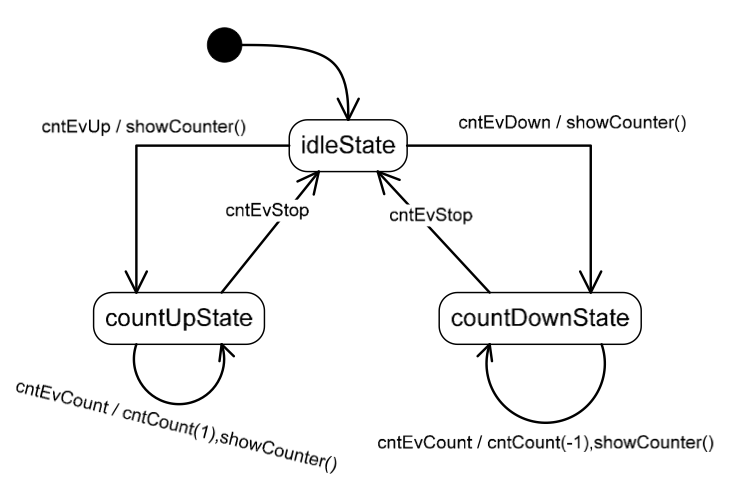
\includegraphics[scale = 0.4]{images/FSM/Up_down_counter}  
  \caption{Beispiel für die Betrachtungen: Up/Down-Counter (prozedural)}
  \label{fig:up_down_counter}}
\end{figure}
\begin{itemize}
  \item Zustände (States) werden in einem eunum definiert (nicht public!)
\begin{lstlisting}
typdef enum {idleState,         //idle state
             countUpState,      //counting up at each count event
             countDownState}    //counting down at each count event
             State;
\end{lstlisting}
\item Ereignisse (Events) werden in einem enum definiert (public!)
\begin{lstlisting}
typdef enum {cntEvUp,       //count upawards
             cntEvDown,     //count downwards
             cntEvCount,    //count (up or down)
             cntEvStop}     //stop counting
             CntEvent;
\end{lstlisting}
\item Die FSM wird in zwei Funktionen implementiert
\begin{lstlisting}
void cntCtrlInit();
//initalizes counter FSM

void cntCtrlProcess(CntEvent e);
//changes the state of the FSM based on the event 'e'
//starts the actions
\end{lstlisting}


\item Der aktuelle Zustand der FSM wird in einer statischen Variablen gehalten
\begin{lstlisting}
typdef enum {idleState,         //idle state
             countUpState,      //counting up at each count event
             countDownState}    //counting down at each count event
             State;
             
static State currentState = idlState; //current state of the FSM

void cntCtrlInit()
{
  currentState = idleState; //init state
  cntInit(0);
}
\end{lstlisting}

\end{itemize}

\subsubsection{Vollständiger Code für prozedurales Steuerkonstrukt}
\begin{lstlisting}
// counterCtrl.h
//
// implements the Finite State Machine (FSM) of an up/down-Counter
//
// (C) R. Bonderer, HSR Hochschule Rapperswil, Nov. 2010
//

#ifndef COUNTERCTRL_H__
#define COUNTERCTRL_H__

typedef enum {cntEvUp,       // count upwards
              cntEvDown,     // count downwards
              cntEvCount,    // count (up or down)
              cntEvStop}     // stop counting
             CntEvent;

void cntCtrlInit();
// initializes counter FSM

void cntCtrlProcess(CntEvent e);
// changes the state of the FSM based on the event 'e'
// starts the actions

#endif
\end{lstlisting}
\begin{lstlisting}
// counterCtrl.c
//
// implements the Finite State Machine (FSM) of an up/down-Counter
//
// (C) R. Bonderer, HSR Hochschule Rapperswil, Okt. 2011
//

#include <stdio.h>
#include "counterCtrl.h"
#include "counter.h"

typedef enum {idleState,        // idle state
              countUpState,     // counting up at each count event
              countDownState}   // counting down at each count event
             State;

static State currentState = idleState; // holds the current state of the FSM

void cntCtrlInit()
{
  currentState = idleState;
  cntInit(0);
}


void cntCtrlProcess(CntEvent e)
{
  switch (currentState)
  {
    case idleState:
      printf("State: idleState\n");
      if (cntEvUp == e)
      {
        // actions
        printf("State: idleState, counter = %d\n", cntGetCounter());
        // state transition
        printf("Changing to State: countUpState\n");
        currentState = countUpState;
      }
      if (cntEvDown == e)
      {
        // actions
        printf("State: idleState, counter = %d\n", cntGetCounter());
        // state transition
        printf("Changing to State: countDownState\n");
        currentState = countDownState;
      }
      break;
      
    case countUpState:
      printf("State: countUpState\n");
      if (cntEvCount == e)
      {
        // actions
        cntCount(1);
        printf("State: countUpState, counter = %d\n", cntGetCounter());
        // state transition
      }
      if (cntEvStop == e)
      {
        // actions
        // state transition
        printf("Changing to State: idleState\n");
        currentState = idleState;
      }
      break;
      
    case countDownState:
      printf("State: countDownState\n");
      if (cntEvCount == e)
      {
        // actions
        cntCount(-1);
        printf("State: countDownState, counter = %d\n", cntGetCounter());
        // state transition
      }
      if (cntEvStop == e)
      {
        // actions
        // state transition
        printf("Changing to State: idleState\n");
        currentState = idleState;
      }
      break;
      
    default:
      break;
  }
}
\end{lstlisting}

\begin{lstlisting}
// counterTest.c
//
// Test program for the Finite State Machine (FSM) of an up/down-Counter
//
// (C) R. Bonderer, HSR Hochschule Rapperswil, Nov. 2010
//

#include <stdio.h>
#include "counterCtrl.h"

int main(void)
{
  char answer;
  
  cntCtrlInit();
  
  do
  {
    printf("\n-------------------------------------------\n");
    printf("    u   Count up\n");
    printf("    d   Count down\n");
    printf("    c   Count\n");
    printf("    s   Stop counting\n");
    printf("    q   Quit\n");

    printf("\nPlease press key: ");
    scanf("%c", &answer);
    getchar();  // nach scanf() ist noch ein '\n' im Inputbuffer: auslesen und wegwerfen

    printf("\n");
    
    switch (answer)
    {
      case 'u':
        cntCtrlProcess(cntEvUp);
        break;
      case 'd':
        cntCtrlProcess(cntEvDown);
        break;
      case 'c':
        cntCtrlProcess(cntEvCount);
        break;
      case 's':
        cntCtrlProcess(cntEvStop);
        break;
      default:
        break;
    }
  } while (answer != 'q');
  
  return 0;
}
\end{lstlisting}

\subsubsection{Realisierung mit Steuerkonstrukt (Objektorientiert in
C++)\buch{p.21}}

\begin{figure}[h]
  \centering
  {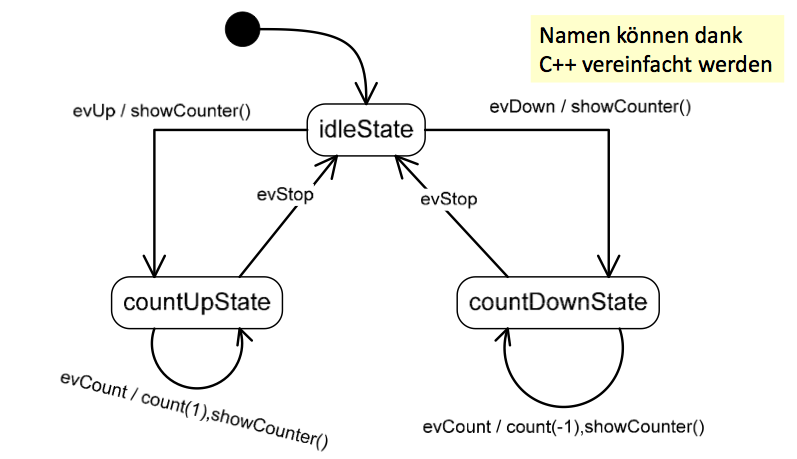
\includegraphics[scale = 0.4]{images/FSM/Up_down_counter_obj}  
  \caption{Beispiel für die Betrachtungen: Up/Down-Counter (objektorientiert)}
  \label{fig:up_down_counter_obj}}
\end{figure}

\begin{itemize}
  \item Logisch gesehen funktioniert die objektorientierte Variante völlig
  identisch wie die prozedurale
  \item Dank des Klassenkonstrukts kann die FSM sauber gekapselt werden
  \item Mehrere Instanzen derselben FSM können einfach erstellt werden
  \item Ein Modulkürzel ist nicht notwendig, da alle Namen im Kontext von
  Klassen definiert werden
  \item Der Code wird eleganter, eine Performanceeinbusse ist nicht vorhanden
  \item States werden im \textbf{privaten-Teil} der Klasse mit einem enum
  definiert
\begin{lstlisting}
enum State {idleState,        // idle state 
            countUpState,     // counting up at each count event 
            countDownState};  //counting down at each count event
\end{lstlisting}
\item Events werden im \textbf{public-Teil} der klasse mit einem enum definiert
(public, weil die Events zur Schnittstelle gehören)
\begin{lstlisting}
enum Event {evUp,     // count upwards
            evDown,   // count downwards 
            evCount,  // count (up or down)
            evStop};  // stop counting
\end{lstlisting}
\item Die FSM wird in zwei Funktionen implementiert
\begin{lstlisting}
CounterCtrl::CounterCtrl(); 
// Ctor initializes counter FSM

void CounterCtrl::process(CounterCtrl::Event e); 
// changes the state of the FSM based on the event 'e' 
// starts the actions
\end{lstlisting}
\item Der aktuelle Zustand der FSM (currentState wird in einem Attribut der
Klasse gehalten)
\begin{figure}[h]
  \centering
  {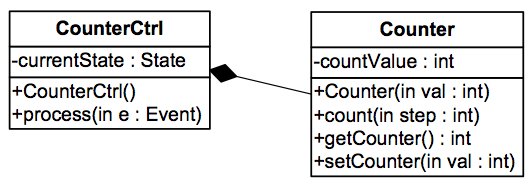
\includegraphics[scale = 0.4]{images/FSM/klasseCounter}  
  \caption{Klasse Counter}
  \label{fig:klasseCounter}}
\end{figure}
\item \textbf{Entry-Actions} müssen überall dor hinzugefügt werden, wo in einen
neuen Zustand gewechselt wird. Üblicherweise muss die Entry-Action für einen
bestimmten Zustand bei mehreren Transitionen codiert werden.
\item \textbf{Exit-Actions} müssen überall dort hinzugefügt werden, wo ein
Zustand verlassen, d.h. in einen anderen Zustand gewechselt, wird. Üblicherweise
muss die Exit-Action für einen bestimmten Zustand bei mehreren Transitionen
codiert werden.
\end{itemize}

\subsubsection{Vollständiger Code für objektorientiertes Steuerkonstrukt}
\begin{lstlisting}
// counterCtrl.h
//
// implements the Finite State Machine (FSM) of an up/down-Counter
//
// (C) R. Bonderer, HSR Hochschule Rapperswil, Nov. 2010
//

#ifndef COUNTERCTRL_H__
#define COUNTERCTRL_H__
#include "counter.h"

class CounterCtrl
{
  public:
    enum Event{evUp,       // count upwards
               evDown,     // count downwards
               evCount,    // count (up or down)
               evStop};    // stop counting
    CounterCtrl();
    void process(Event e);
    // changes the state of the FSM based on the event 'e'
    // starts the actions

  private:
    enum State{idleState,        // idle state
               countUpState,     // counting up at each count event
               countDownState};  // counting down at each count event

    State currentState;     // holds the current state of the FSM
    Counter myCounter;
};
#endif
\end{lstlisting}

\begin{lstlisting}
// counterCtrl.cpp
//
// implements the Finite State Machine (FSM) of an up/down-Counter
//
// (C) R. Bonderer, HSR Hochschule Rapperswil, Okt. 2011
//

#include <iostream>
#include "counterCtrl.h"
#include "counter.h"
using namespace std;

CounterCtrl::CounterCtrl() : 
  currentState(idleState),
  myCounter(0)
{
}

void CounterCtrl::process(Event e)
{
  switch (currentState)
  {
    case idleState:
      cout << "State: idleState" << endl;
      if (evUp == e)
      {
        // actions
        cout << "State: idleState, counter = " << myCounter.getCounter() << endl;
        // state transition
        cout << "Changing to State: countUpState" << endl;
        currentState = countUpState;
      }
      if (evDown == e)
      {
        // actions
        cout << "State: idleState, counter = " << myCounter.getCounter() << endl;
        // state transition
        cout << "Changing to State: countDownState" << endl;
        currentState = countDownState;
      }
      break;
      
    case countUpState:
      cout << "State: countUpState" << endl;
      if (evCount == e)
      {
        // actions
        myCounter.count(1);
        cout << "State: countUpState, counter = " << myCounter.getCounter() << endl;
        // state transition
      }
      if (evStop == e)
      {
        // actions
        // state transition
        cout << "Changing to State: idleState" << endl;
        currentState = idleState;
      }
      break;
      
    case countDownState:
      cout << "State: countDownState" << endl;
      if (evCount == e)
      {
        // actions
        myCounter.count(-1);
        cout << "State: countDownState, counter = " << myCounter.getCounter() << endl;
        // state transition
      }
      if (evStop == e)
      {
        // actions
        // state transition
        cout << "Changing to State: idleState" << endl;
        currentState = idleState;
      }
      break;
      
    default:
      break;
  }
}
\end{lstlisting}

\begin{lstlisting}
// counter.h
//
// implements an up/down-Counter
//
// (C) R. Bonderer, HSR Hochschule Rapperswil, Nov. 2010
//

#ifndef COUNTER_H__
#define COUNTER_H__

class Counter
{
  public:
    Counter(int val);

    void count(int step);
    // counts the counter up (step>0) or down (step<0) by step

    int getCounter() const;
    // returns the counter value

    void setCounter(int val);
    // sets the counter to val
  private:
    int countValue;
};

#endif
\end{lstlisting}

\begin{lstlisting}
// counter.cpp
//
// implements an up/down-Counter
//
// (C) R. Bonderer, HSR Hochschule Rapperswil, Nov. 2010
//

#include "counter.h"

Counter::Counter(int val): countValue(val)
{
}

void Counter::count(int step)
{
  countValue += step;
}

int Counter::getCounter() const
{
  return countValue;
}

void Counter::setCounter(int val)
{
  countValue = val;
}
\end{lstlisting}

\begin{lstlisting}
// counterTest.cpp
//
// Test program for the Finite State Machine (FSM) of an up/down-Counter
//
// (C) R. Bonderer, HSR Hochschule Rapperswil, Nov. 2010
//

#include <iostream>
#include "counterCtrl.h"
using namespace std;

int main(void)
{
  char answer;
  CounterCtrl myFsm;
  
  do
  {
    cout << endl << "-------------------------------------------" << endl;
    cout << "    u   Count up" << endl;
    cout << "    d   Count down" << endl;
    cout << "    c   Count" << endl;
    cout << "    s   Stop counting" << endl;
    cout << "    q   Quit" << endl;

    cout << endl << "Please press key: ";
    cin >> answer;
    cout << endl;
    
    switch (answer)
    {
      case 'u':
        myFsm.process(CounterCtrl::evUp);
        break;
      case 'd':
        myFsm.process(CounterCtrl::evDown);
        break;
      case 'c':
        myFsm.process(CounterCtrl::evCount);
        break;
      case 's':
        myFsm.process(CounterCtrl::evStop);
        break;
      default:
        break;
    }
  } while (answer != 'q');
  
  return 0;
}
\end{lstlisting}

\subsubsection{Realisierung mit Tabelle\buch{p.33}}
\begin{itemize}
  \item Die objektorientierte Variante verwendet einzig die Datenkapselung,
  Vererbung und Polymorphismus werden nicht benötigt
  \item Die objektorientierte Variante kann klarer und schäner strukturiert
  implementiert werden. Im folgenden wird nur diese Variante gezeigt, die
  C-Version kann jedoch einfach davon abgeleitet werden
  \item Die ganze FSM ist in einer Tabelle gespeichert
  \item Die Aktionen sind als Funktionen implementiert, in der Tabelle steht der
  entsprechende Funktionspointer
  \item Die Abarbeitung der FSM erfolgt mit Hilfe einer \textit{Execution
  Engine}, die in der Tabelle "`nachschaut"', was zu tun ist
  \item Die Execution Engine ändert sich nicht, wenn die FSM geändert wird
  \item Das Testprogramm ist völlig unverändert
  \item Die Schnittstell von CounterCtrl (public-Teil) ist ebenfalls identisch
  \item Die Klasse Counter ändert auch nicht
  \item Die \textbf{einzige Änderung} liegt im privaten Teil der
  CounterCtrl-Klasse und natürlich in deren Implementation
  \item Alle (Tansitions-)Aktionen werden als Methoden deklariert,
  \textit{Action} wird als Funktionspointer definiert. Diese Methoden müssen
  alle mit dem Funktionspointer übereinstimmen
 \begin{lstlisting}
 typedef void (CounterCtrl::*Action)(void);// ptr for action function
  // action functions 
  void actionIdleUp(void); 
  void actionIdleDown(void); 
  void actionDoNothing(void); 
  void actionUpUp(void); 
  void actionDownDown(void);
 \end{lstlisting}
 \item Die Transition wird als klasseninterne Struktur deklariert. Sie besteht
 aus
 \begin{itemize}
   \item Aktueller Zustand
   \item Event
   \item Funktionspointer auf Aktionsmethode
   \item Nächster Zustand
 \end{itemize}
fsm() wird als statischer Array deklariert.
\begin{lstlisting}
struct Transition
    {
      State currentState;   // current state
      Event ev;             // event triggering the transition
      Action pAction;       // pointer to action function
      State nextState;      // next state
    };
    static const Transition fsm[];
\end{lstlisting}
\item Tabellendefinition in CounterCtrl.cpp
\begin{figure}[h]
  \centering
  {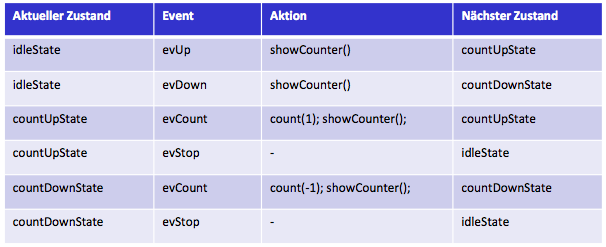
\includegraphics[scale = 0.4]{images/FSM/tabelle}  
  \caption{Tabellendefinition}
  \label{fig:tabelle}}
\end{figure}
\begin{lstlisting}
enum {transCount = 6}; // number of transitions (rows in following table)
const CounterCtrl::Transition CounterCtrl::fsm[transCount] =  // this table defines the fsm
{//currentState     triggering event  action function                 next state
  {idleState,       evUp,             &CounterCtrl::actionIdleUp,     countUpState},
  {idleState,       evDown,           &CounterCtrl::actionIdleDown,   countDownState},
  {countUpState,    evCount,          &CounterCtrl::actionUpUp,       countUpState},
  {countUpState,    evStop,           &CounterCtrl::actionDoNothing,  idleState},
  {countDownState,  evCount,          &CounterCtrl::actionDownDown,   countDownState},
  {countDownState,  evStop,           &CounterCtrl::actionDoNothing,  idleState}
};
\end{lstlisting}
\item Aufbau einer Aktionsmethode
\begin{lstlisting}
void CounterCtrl::actionDownDown(void)
{
  myCounter.count(-1);
  cout << "State: countDownState, counter = " << myCounter.getCounter() << endl;
}
\end{lstlisting}
\item Execution Engine
\begin{lstlisting}
void CounterCtrl::process(Event e)    // execution engine, this function never changes
{
  for (int i=0; i<transCount; i++)
  {
    if (fsm[i].currentState == currentState &&  fsm[i].ev == e) // is there an entry in the table?
    {
      (this->*fsm[i].pAction)();
      currentState = fsm[i].nextState;
      break;
    }
  }
}
\end{lstlisting}
\item Wenn der Zustandsübergang nicht nur durch einen Event, sondern eine
komplexe Prüfung (Event und Guard) ausgelöst wird, dann könnte der Eventeintrag
in der Tabelle durch einen weiteren Funktionspointer auf eine Checkfunktion
ersetzt werden
\begin{lstlisting}
typedef bool (CounterCtrl::*Checker)(Event);
// function ptr for checker function 
// checker functions
bool checkIdleUp(Event check); 
...

struct Transition 
{
  State currentState; // current state
  Checker pChecker;   // pointer to checker function
  Action pAction;     // pointer to action function
  State nextState;    // next state
};
\end{lstlisting}
\end{itemize}

\subsubsection{Vollständiger Code für Tabellen-Realisation}
\begin{lstlisting}
// counterCtrl.h
//
// implements the Finite State Machine (FSM) of an up/down-Counter as a table
//
// (C) R. Bonderer, HSR Hochschule Rapperswil, Okt. 2011
//

#ifndef COUNTERCTRL_H__
#define COUNTERCTRL_H__
#include "counter.h"

class CounterCtrl
{
  public:
    enum Event{evUp,       // count upwards
               evDown,     // count downwards
               evCount,    // count (up or down)
               evStop};    // stop counting
    CounterCtrl();
    void process(Event e);
    // changes the state of the FSM based on the event 'e'
    // starts the actions

  private:
    enum State{idleState,         // idle state
               countUpState,      // counting up at each count event
               countDownState};   // counting down at each count event

    State currentState;           // holds the current state of the FSM
    Counter myCounter;
    
    typedef bool (CounterCtrl::*Checker)(Event); // function ptr for checker function
    typedef void (CounterCtrl::*Action)(void);   // function ptr for action function
    // check functions
    bool checkIdleUp(Event check);
    bool checkIdleDown(Event check);
    bool checkUpIdle(Event check);
    bool checkDownIdle(Event check);
    bool checkUpUp(Event check);
    bool checkDownDown(Event check);
    
    // action functions
    void actionIdleUp(void);
    void actionIdleDown(void);
    void actionUpIdle(void);
    void actionDownIdle(void);
    void actionUpUp(void);
    void actionDownDown(void);
    
    struct Transition
    {
      State currentState;   // current state
      Checker pChecker;     // pointer to checker function
      Action pAction;       // pointer to action function
      State nextState;      // next state
    };
    static const Transition fsm[];
};
#endif
\end{lstlisting}

\begin{lstlisting}
//
// counterCtrl.cpp
//
// implements the Finite State Machine (FSM) of an up/down-Counter as a table
//
// (C) R. Bonderer, HSR Hochschule Rapperswil, Okt. 2011
//

#include <iostream>
#include "counterCtrl.h"
#include "counter.h"
using namespace std;

enum {transCount = 6}; // number of transitions (rows in following table)
const CounterCtrl::Transition CounterCtrl::fsm[transCount] =  // this table defines the fsm
{//currentState     checker function              action function               next state
  {idleState,       &CounterCtrl::checkIdleUp,    &CounterCtrl::actionIdleUp,   countUpState},
  {idleState,       &CounterCtrl::checkIdleDown,  &CounterCtrl::actionIdleDown, countDownState},
  {countUpState,    &CounterCtrl::checkUpUp,      &CounterCtrl::actionUpUp,     countUpState},
  {countUpState,    &CounterCtrl::checkUpIdle,    &CounterCtrl::actionUpIdle,   idleState},
  {countDownState,  &CounterCtrl::checkDownDown,  &CounterCtrl::actionDownDown, countDownState},
  {countDownState,  &CounterCtrl::checkDownIdle,  &CounterCtrl::actionDownIdle, idleState}
};

CounterCtrl::CounterCtrl() : 
  currentState(idleState),
  myCounter(0)
{
}

void CounterCtrl::process(Event e)    // this function never changes
{
  for (int i=0; i<transCount; i++)
  {
    if (fsm[i].currentState == currentState &&  // is there an entry in the table?
      (this->*fsm[i].pChecker)(e))
    {
      (this->*fsm[i].pAction)();
      currentState = fsm[i].nextState;
      break;
    }
  }
}

// check functions
bool CounterCtrl::checkIdleUp(Event check)
{
  return evUp == check;
}

bool CounterCtrl::checkIdleDown(Event check)
{
  return evDown == check;
}

bool CounterCtrl::checkUpIdle(Event check)
{
  return evStop == check;
}

bool CounterCtrl::checkDownIdle(Event check)
{
  return evStop == check;
}

bool CounterCtrl::checkUpUp(Event check)
{
  return evCount == check;
}

bool CounterCtrl::checkDownDown(Event check)
{
  return evCount == check;
}

// action functions
void CounterCtrl::actionIdleUp(void)
{
  cout << "State: idleState, counter = " << myCounter.getCounter() << endl;
}

void CounterCtrl::actionIdleDown(void)
{
  cout << "State: idleState, counter = " << myCounter.getCounter() << endl;
}

void CounterCtrl::actionUpIdle(void)
{
}

void CounterCtrl::actionDownIdle(void)
{
}

void CounterCtrl::actionUpUp(void)
{
  myCounter.count(1);
  cout << "State: countUpState, counter = " << myCounter.getCounter() << endl;
}

void CounterCtrl::actionDownDown(void)
{
  myCounter.count(-1);
  cout << "State: countDownState, counter = " << myCounter.getCounter() << endl;
}

\end{lstlisting}

\begin{lstlisting}
//
// counter.h
//
// implements an up/down-Counter
//
// (C) R. Bonderer, HSR Hochschule Rapperswil, Nov. 2010
//

#ifndef COUNTER_H__
#define COUNTER_H__

class Counter
{
  public:
    Counter(int val);

    void count(int step);
    // counts the counter up (step>0) or down (step<0) by step

    int getCounter() const;
    // returns the counter value

    void setCounter(int val);
    // sets the counter to val
  private:
    int countValue;
};

#endif

\end{lstlisting}
\begin{lstlisting}
//
// counter.cpp
//
// implements an up/down-Counter
//
// (C) R. Bonderer, HSR Hochschule Rapperswil, Nov. 2010
//

#include "counter.h"

Counter::Counter(int val): countValue(val)
{
}

void Counter::count(int step)
{
  countValue += step;
}

int Counter::getCounter() const
{
  return countValue;
}

void Counter::setCounter(int val)
{
  countValue = val;
}

\end{lstlisting}

\begin{lstlisting}
//
// counterTest.cpp
//
// Test program for the Finite State Machine (FSM) of an up/down-Counter
//
// (C) R. Bonderer, HSR Hochschule Rapperswil, Nov. 2010
//

#include <iostream>
#include "counterCtrl.h"
using namespace std;

int main(void)
{
  char answer;
  CounterCtrl myFsm;
  
  do
  {
    cout << endl << "-------------------------------------------" << endl;
    cout << "    u   Count up" << endl;
    cout << "    d   Count down" << endl;
    cout << "    c   Count" << endl;
    cout << "    s   Stop counting" << endl;
    cout << "    q   Quit" << endl;

    cout << endl << "Please press key: ";
    cin >> answer;
    cout << endl;
    
    switch (answer)
    {
      case 'u':
        myFsm.process(CounterCtrl::evUp);
        break;
      case 'd':
        myFsm.process(CounterCtrl::evDown);
        break;
      case 'c':
        myFsm.process(CounterCtrl::evCount);
        break;
      case 's':
        myFsm.process(CounterCtrl::evStop);
        break;
      default:
        break;
    }
  } while (answer != 'q');
  
  return 0;
}

\end{lstlisting}

\subsubsection{Realisierung mit State Pattern\buch{p.3}}
\begin{itemize}
  \item Das Prinzip besteht aus einer abstrakten State-Basisklasse. Pro Zustand
  muss eine eigene Klasse definiert werden, die von dieser abstrakten
  Basisklasse erbt.
  \item Die Realisierung nutzt das Polymorphismus-Konzept, jede konkrete
  State-Klasse ist ein \textit{Singleton}
  \item Statt lange switch-case-if-Konstrukte wird beim State Pattern ein
  bestimmter Zustand vollständig in einer eigenen Klasse realisiert. Die Logik
  wird somit aufgeteilt.
  \item \textbf{Context} definiert die interessierenden Schnittstellen für
  Clients, unterhält eine Instanz einer konkreten Unterklasse von State, die den
  aktuellen Zustand definiert, bzw. repräsentiert
  \item \textbf{State} definiert eine schnittstelle zur FMS in Form einer
  abstrakten Klasse
  \item \textbf{ConcreteStateX Unterklassen} jede Unterklasse implementiert
  genau einen Zustand (ist Singleton)
 \begin{figure}[h]
  \centering
  {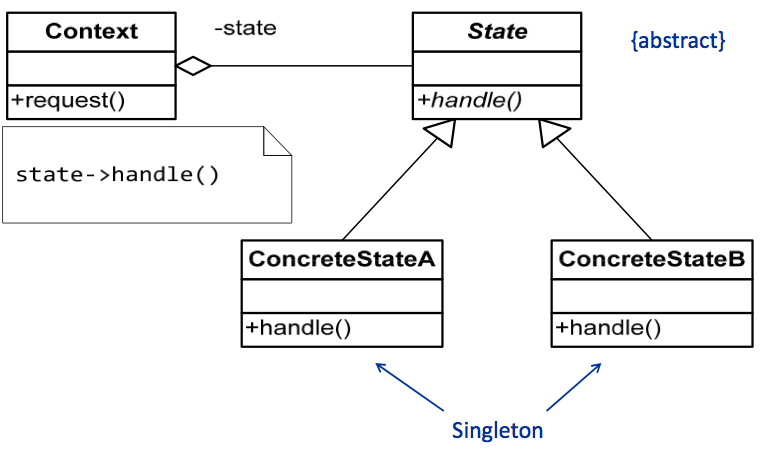
\includegraphics[scale = 0.4]{images/FSM/state_pattern}  
  \caption{Teile des State Pattern}
  \label{fig:state_pattern}}
\end{figure}
\item Das State Pattern definiert die Zuständigkeit nicht
\item Die Transitionen könnten in der Context-Klasse definiert werden. Der
Nachteil dieser Variante ist, dass dort zentral sehr viel Intelligenz vorhanden
sein müsste. Da diese Klasse auch den Zugriff zur Aussenwelt darstellt, sollte
sie möglichst schlank sein.
\item Die bessere Variante ist, wenn die State-Klassen auch gleich ihre
Transitionen realisieren. Diese Variante wird oft mittels friend-Deklaration
realisiert
\item Im folgenden betrachten wir eine saubere Lösung ohne friend-Deklaration.
 \begin{figure}[h]
  \centering
  {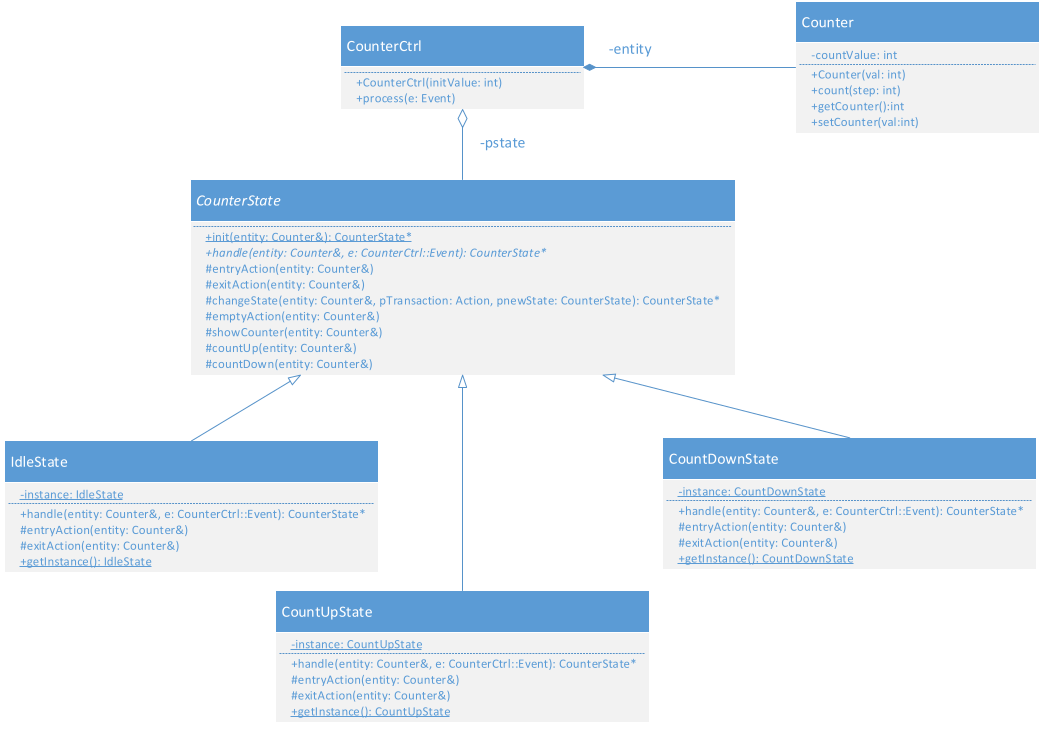
\includegraphics[scale = 0.4]{images/FSM/klassendiagramm}  
  \caption{Klassendiagramm des Counters mit dem State Pattern}
  \label{fig:klassendiagramm}}
\end{figure}
\item counterCtrl.h : Schnittstelle zur FSM
\begin{lstlisting}
// counterCtrl.h
//
// implements the Finite State Machine (FSM) of an up/down-Counter
//
// (C) R. Bonderer, HSR Hochschule Rapperswil, Oct. 2011
//

#ifndef COUNTERCTRL_H__
#define COUNTERCTRL_H__

class CounterState;   // forward declaration

class CounterCtrl
// this is the 'Context' class of the State pattern
{
  public:
    enum Event{evUp,       // count upwards
               evDown,     // count downwards
               evCount,    // count (up or down)
               evStop};    // stop counting
    CounterCtrl();
    void process(Event e);  
    // changes the state of the FSM based on the event 'e'
  private:
    CounterState* pState;
};
#endif
\end{lstlisting}
\item counterCtrl.cpp
\begin{lstlisting}
// counterCtrl.cpp
//
// implements the Finite State Machine (FSM) of an up/down-Counter
// CounterCtrl is the Context class in the State pattern
//
// (C) R. Bonderer, HSR Hochschule Rapperswil, Oct. 2011
//

#include "counterCtrl.h"
#include "counterState.h"

CounterCtrl::CounterCtrl()
{
  pState = IdleState::getInstance(); // initial state
}

void CounterCtrl::process(Event e)
{ // delegates all requests to CounterState
  pState =  pState->process(e);
}
\end{lstlisting}
\item class CounterState: Interface
\begin{lstlisting}
//
// counterState.h
//
// implements an up/down-Counter
// this file contains all classes of the state machine
// it may make sense to have separate files for each state
//
// (C) R. Bonderer, HSR Hochschule Rapperswil, Oct. 2011
//

#ifndef COUNTERSTATE_H__
#define COUNTERSTATE_H__
#include "counterctrl.h"

class Counter;

class CounterState  // abstract base class
{
  public:
    virtual CounterState* process(CounterCtrl::Event e) = 0;
    // returns new state
  protected:
    virtual void entryAction(void) = 0;
    virtual void exitAction(void) = 0;
    typedef void (CounterState::*Action)(void);   // ptr to action function
    CounterState* changeState(Action ptransAction, CounterState* pnewState);

    // transition actions
    void emptyAction() {};
    void showCounter();
    void countUp();
    void countDown();

    static Counter myCounter;
};

class IdleState : public CounterState // it's a singleton
{
  public:
    static IdleState* getInstance();
    virtual CounterState*  process(CounterCtrl::Event e);
  protected:
    virtual void entryAction(void);
    virtual void exitAction(void);
  private:
    IdleState() {};
    static IdleState instance;
};

class CountUpState : public CounterState // it's a singleton
{
  public:
    static CountUpState* getInstance();
    virtual CounterState*  process(CounterCtrl::Event e);
  protected:
    virtual void entryAction(void);
    virtual void exitAction(void);
  private:
    CountUpState() {};
    static CountUpState instance;
};

class CountDownState : public CounterState // it's a singleton
{
  public:
    static CountDownState* getInstance();
    virtual CounterState*  process(CounterCtrl::Event e);
  protected:
    virtual void entryAction(void);
    virtual void exitAction(void);
  private:
    CountDownState() {};
    static CountDownState instance;
};
#endif

\end{lstlisting}
\item class CountUpState: Implementation
\begin{lstlisting}
//
// counterState.cpp
//
// implements all states of an up/down-Counter
// this file contains all classes of the state machine.
// it may make sense to have separate files for each state
//
// (C) R. Bonderer, HSR Hochschule Rapperswil, Oct. 2011
//

#include <iostream>
#include "counterState.h"
#include "counterCtrl.h"
#include "counter.h"
using namespace std;


//class CounterState
Counter CounterState::myCounter(0);  // initialize static data

CounterState* CounterState::changeState(Action ptransAction, CounterState* pnewState)
{
  exitAction();              // polymorphic call of exit action
  (this->*ptransAction)();   // call of transition action
  pnewState->entryAction();  // polymorphic call of entry action
  return pnewState;
}

void CounterState::showCounter()
{
  cout << "counter = " << myCounter.getCounter() << endl;
}

void CounterState::countUp()
{
  myCounter.count(1);
  cout << "counter = " << myCounter.getCounter() << endl;
}

void CounterState::countDown()
{
  myCounter.count(-1);
  cout << "counter = " << myCounter.getCounter() << endl;
}


// class IdleState
IdleState IdleState::instance;
IdleState* IdleState::getInstance()
{
  return &instance;
}

CounterState* IdleState::process(CounterCtrl::Event e)
{
  cout << "State: idleState" << endl;
  if (CounterCtrl::evUp == e)
  {
    // state transition
    return changeState(&IdleState::countUp, CountUpState::getInstance());
  }
  if (CounterCtrl::evDown == e)
  {
    // state transition
    return changeState(&IdleState::showCounter, CountDownState::getInstance());
  }
  return this;
}

void IdleState::entryAction(void)
{
  cout << "Enter idleState" << endl;
}

void IdleState::exitAction(void)
{
  cout << "Exit from idleState" << endl;
}


// class CountUpState
CountUpState CountUpState::instance;
CountUpState* CountUpState::getInstance()
{
  return &instance;
}

CounterState* CountUpState::process(CounterCtrl::Event e)
{
  cout << "State: countUpState" << endl;
  if (CounterCtrl::evCount == e)
  {
    // state transition
    return changeState(&CountUpState::countUp, CountUpState::getInstance());
  }
  if (CounterCtrl::evStop == e)
  {
    // state transition
    return changeState(&CountUpState::emptyAction, IdleState::getInstance());
  }
  return this;
}

void CountUpState::entryAction(void)
{
  cout << "Enter countUpState" << endl;
}

void CountUpState::exitAction(void)
{
  cout << "Exit from countUpState" << endl;
}

// class CountDownState
CountDownState CountDownState::instance;
CountDownState* CountDownState::getInstance()
{
  return &instance;
}

CounterState* CountDownState::process(CounterCtrl::Event e)
{
  cout << "State: countDownState" << endl;
  if (CounterCtrl::evCount == e)
  {
    // state transition
    return changeState(&CountDownState::countDown, CountDownState::getInstance());
  }
  if (CounterCtrl::evStop == e)
  {
    // state transition
    return changeState(&CountDownState::emptyAction, IdleState::getInstance());
  }
  return this;
}

void CountDownState::entryAction(void)
{
  cout << "Enter countDownState" << endl;
}

void CountDownState::exitAction(void)
{
  cout << "Exit from countDownState" << endl;
}

\end{lstlisting}
\item counter.h
\begin{lstlisting}
//
// counter.h
//
// implements an up/down-Counter
//
// (C) R. Bonderer, HSR Hochschule Rapperswil, Nov. 2010
//

#ifndef COUNTER_H__
#define COUNTER_H__

class Counter
{
  public:
    Counter(int val=0);

    void count(int step);
    // counts the counter up (step>0) or down (step<0) by step

    int getCounter() const;
    // returns the counter value

    void setCounter(int val);
    // sets the counter to val
  private:
    int countValue;
};

#endif

\end{lstlisting}
\item counter.cpp
\begin{lstlisting}
//
// counter.cpp
//
// implements an up/down-Counter
//
// (C) R. Bonderer, HSR Hochschule Rapperswil, Nov. 2010
//

#include "counter.h"

Counter::Counter(int val): countValue(val)
{
}

void Counter::count(int step)
{
  countValue += step;
}

int Counter::getCounter() const
{
  return countValue;
}

void Counter::setCounter(int val)
{
  countValue = val;
}

\end{lstlisting}
\item counterTest.cpp
\begin{lstlisting}
//
// counterTest.cpp
//
// Test program for the Finite State Machine (FSM) of an up/down-Counter
//
// (C) R. Bonderer, HSR Hochschule Rapperswil, Nov. 2010
//

#include <iostream>
#include "counterCtrl.h"
using namespace std;

int main(void)
{
  char answer;
  CounterCtrl myFsm;
  
  do
  {
    cout << endl << "-------------------------------------------" << endl;
    cout << "    u   Count up" << endl;
    cout << "    d   Count down" << endl;
    cout << "    c   Count" << endl;
    cout << "    s   Stop counting" << endl;
    cout << "    q   Quit" << endl;

    cout << endl << "Please press key: ";
    cin >> answer;
    cout << endl;
    
    switch (answer)
    {
      case 'u':
        myFsm.process(CounterCtrl::evUp);
        break;
      case 'd':
        myFsm.process(CounterCtrl::evDown);
        break;
      case 'c':
        myFsm.process(CounterCtrl::evCount);
        break;
      case 's':
        myFsm.process(CounterCtrl::evStop);
        break;
      default:
        break;
    }
  } while (answer != 'q');
  
  return 0;
}


\end{lstlisting}
\end{itemize}
